\documentclass[10pt,letterpaper]{article}
\usepackage[top=0.85in,left=1.25in,footskip=0.75in,marginparwidth=2in]{geometry}

% use Unicode characters - try changing the option if you run into troubles with special characters (e.g. umlauts)
\usepackage[utf8]{inputenc}

% clean citations
\usepackage[style=authoryear,sorting=nyt,natbib, backend=biber, maxbibnames=20, maxcitenames=1, dashed=false, uniquelist=false]{biblatex}
\addbibresource{library.bib}


% hyperref makes references clicky. use \url{www.example.com} or \href{www.example.com}{description} to add a clicky url
\usepackage{nameref,hyperref}

% line numbers
\usepackage[right]{lineno}

% improves typesetting in LaTeX
\usepackage{microtype}
\DisableLigatures[f]{encoding = *, family = * }

% text layout - change as needed
\raggedright
\setlength{\parindent}{0.5cm}
\textwidth 6.0in 
\textheight 8.75in

% Remove % for double line spacing
%\usepackage{setspace} 
%\doublespacing

% use adjustwidth environment to exceed text width (see examples in text)
\usepackage{changepage}
\usepackage{setspace}

% adjust caption style
\usepackage[aboveskip=1pt,labelfont=bf,labelsep=period,singlelinecheck=off]{caption}

% remove brackets from references
\makeatletter
\renewcommand{\@biblabel}[1]{\quad#1.}
\makeatother

% headrule, footrule and page numbers
\usepackage{lastpage,fancyhdr,graphicx}
\usepackage{epstopdf}
\pagestyle{myheadings}
\pagestyle{fancy}
\fancyhf{}
\rfoot{\thepage/\pageref{LastPage}}
\renewcommand{\footrule}{\hrule height 0pt \vspace{2mm}}
\fancyheadoffset[L]{2.25in}
\fancyfootoffset[L]{2.25in}

% use \textcolor{color}{text} for colored text (e.g. highlight to-do areas)
\usepackage{color}
\usepackage[table]{xcolor} % to color the array in a table

% define custom colors (this one is for figure captions)
\definecolor{Gray}{gray}{.25}

% this is required to include graphics
\usepackage{graphicx}

\usepackage{multirow}

% use if you want to put caption to the side of the figure - see example in text
\usepackage{sidecap}

% use for have text wrap around figures
\usepackage{wrapfig}
\usepackage[pscoord]{eso-pic}
\usepackage[fulladjust]{marginnote}
\reversemarginpar
% use for flush all figures to the end of the pdf document
%\usepackage[nomarkers,figuresonly]{endfloat}

% document begins here
\begin{document}
\vspace*{0.35in}
\justify

\pagestyle{empty} %empty page numbers
% title goes here:
\begin{flushleft}
{\Large
\textbf{Genome-wide association and gene network analysis for starch and protein in sorghum}
}
\doublespacing
\newline
% authors go here:
\\
Sirjan Sapkota\textsuperscript{1,2,*},
Jon Lucas Boatwright\textsuperscript{2},
Kathleen Jordan\textsuperscript{2},
Richard Boyles\textsuperscript{1,3},
Stephen Kresovich\textsuperscript{1,2},
% Author 6\textsuperscript{2},
% Author 7\textsuperscript{1,*}
\\
\bigskip
{1} Department of Plant and Environmental Sciences, Clemson University, Clemson, SC, USA
\\
{2} Advanced Plant Technology Program, Clemson University, Clemson, SC, USA
\\
{3} Pee Dee Research and Education Center, Clemson University, Florence, SC, USA
\\
\bigskip
* correspondence: ssapkot@g.clemson.edu

\end{flushleft}
% now start line numbers
% \linenumbers
\doublespacing
\section*{Abstract}
The grains of cereals are ultimate sink for macromolecules such as starch and protein which serve as principal source of nutrition. Dissection of genetic basis of phenotypic variation for starch and protein is important in metabolic engineering of grain. Genetic studies of starch and protein in sorghum, a cereal crop, has involved single traits and metabolic network involved in their regulation are not completely characterized. In this study we used univariate and multivariate (MV) linear mixed models (LMM) to identify associated genomic regions, potential candidate genes and their interactors. Six single nucleotide polymorphism (SNPs) in strong linkage disequilibrium ($r^2$ \textgreater 0.8) from $\sim$52 Mb of chromosome 8 were significantly associated with starch content. Five of those SNPs were located within mRNA of a heat shock protein 90 (HSP90), \textit{Sobic.008G111600}, with two of them in the coding sequences of the gene. The HSP90 had a total of 142 high confidence (PPI-score: 0.6) first interactors and the network was enriched for six bichemical pathways including protein processing and export. A SNP, S4\_60623675, identified using MV-LMM model was located at 5'UTR of a fatty acid desaturase gene, \textit{Sobic.004G260800}, which interacted with another fatty acid desaturase and several nitrate reductase genes. The two candidates, HSP90 and FAD2, were found to be highly expressed in reproductive tissues. We conclude multivariate analysis of correlated phenotypes can identify biologically important metabolic networks and functional analyses of identified gene candidates can be beneficial in understanding grain filling in sorghum and other cereals.

\section*{Introduction}
The seeds of cereals, that represent an important sink for metabolites during grain filling, are principal source of human and animal nutrition. Sorghum [\textit{Sorghum bicolor}. (L.) Moench] is a cereal crop that provides dietary staple for over half a billion people in semi-arid tropics \parencite{mace2013whole}. While primarily used as animal feed in industrialized economies, the end use products of sorghum grain has diversified to include baking, malting, brewing, and bio-fortification \parencite{zhu2014structure}. Understanding the genetic basis of phenotypic variation in grain composition such as starch and protein could provide the basis for metabolic engineering of these macromolecules through selective breeding.

Linkage mapping has been a powerful method to identify quantitative trait loci (QTL) that cosegregate with a given trait but suffers from two fundamental limitations; only allelic diversity that segregates between the parents can be assayed, and the amount of recombination from bi-parental crosses places a limit on the mapping resolution \parencite{korte2013advantages}. In contrast, genome-wide association studies (GWAS) have mapped genetic variants associated to phenotypes to a much higher resolution using whole genome markers in a diverse group of individuals. The cost effectiveness in generating large scale genotypic data has now led to swathe of GWAS in crops and focus has shifted towards computational challenges \parencite{myles2009association}. Most application of GWAS has focused on single traits, whereas phenotypes are usually correlated and might be controlled by genetic loci with pleiotropic effects. Meanwhile, studies have shown that joint analysis of correlated phenotypes can exploit the correlation among the phenotypes for detecting additional genetic variants with small effects across multiple traits \parencite{korte2012mixed,thoen2017genetic,carlson2019multivariate,rice2020multi}. Some of the approaches to leverage correlation between traits in association analysis include: use of ratios of directly related traits in univariate GWAS \parencite{gieger2008genetics}, combining test statistics from univariate GWAS of each trait to detect pleiotropic effects \parencite{yang2010analyze}, using dimension reduction technique to derive transformed phenotypes for univariate GWAS \parencite{aschard2014maximizing}, and directly modeling multiple traits into a multivariate linear mixed models \parencite{korte2012mixed,zhou2014efficient}.

Association studies for grain quality has been reported in several cereal crops such as maize \parencite{wilson2004dissection,cook2012genetic}, rice \parencite{zhao2011genome,wang2017genome}, sorghum \parencite{sukumaran2012association,rhodes2017genetic}, and wheat \parencite{reif2011association,gaire2019association}. In diverse sorghum accessions, starch and protein show continuous variation ranging from 60 to 72\% and 8 to 18\% of total grain, respectively \parencite{rhodes2017genetic}. Previous association analyses for starch and protein content have identified significantly associated genomic regions in sorghum \parencite{sukumaran2012association,rhodes2017genetic,boyles2017genetic}. Starch and protein content represent majority of grain composition and are likely to be controlled by genetic loci with pleiotropic effects. Such genetic loci could have gone undetected in single trait GWAS, and multivariate GWAS might be able to identify such associations. Furthermore, the path from genetic association to biology is not always straightforward because an association between a genetic variant and a trait may not be informative with respect to the target gene \parencite{gallagher2018post}. In this study, we implemented univariate and multivariate linear mixed models for starch and protein content using sorghum association panel, and identified candidate genes within significantly associated loci. We also performed candidate gene network analysis using protein-protein interaction and studied expression profile of candidate genes and their interactors.

\section*{Materials and Methods}
\label{sec:materials:methods}
\subsection*{Plant material}
A panel of approximately 400 diverse sorghum accessions was planted in randomized complete block design with two replications in 2013, 2014, and 2017 field seasons at the Clemson University Pee Dee Research and Education Center in Florence, SC. This diversity panel, with over 80\% of the accessions from the original United States sorghum association panel (SAP) developed by \citet{casa2008community}, will be referred to as SAP. The details on experimental field design and agronomic practices have been described in details in \citet{boyles2016genome} and \citet{sapkota2020}. Succinctly, the experiments were planted in a two row plots each 6.1 m long, separated by row spacing of 0.762 m with an approximate density of 130,000 plants $ha^{-1}$. Fields were irrigated only when signs of drought stress was seen across the field. Primary panicle of three plants selected from each plot was harvested at physiological maturity. The plants from beginning and end of the row were excluded to account for border effect. Panicles were air dried to a constant moisture (10-12\%) and threshed. A 25g of cleaned and homogenized subsample of grain ground to 1-mm particle size with a CT 193 Cyclotec Sample Mill (FOSS North America) was used in near infrared spectroscopy (NIRS) for compositional analysis.

\subsection*{Phenotypic data}
A DA 7250\texttrademark{} NIR analyzer (Perten Instruments) was used for compositional analysis. The predicted phenotypic values were obtained from the calibrated curves for spectral measurements of ground grain samples. The calibration curve was built using wet chemistry values from a subset of samples. The wet chemistry was performed by Dairyland Laboratories, Inc. (Arcadia, WI) and the Quality Assurance Laboratory at Murphy-Brown, LLC (Warsaw, NC). The details on the prediction curves and wet chemistry can be found in \citet{boyles2017genetic}.

The phenotypic values were fitted into a linear mixed model analysis using lme4 package in R \parencite{lme42015,Rcore2019}. The following mixed model equation was fit:
\begin{equation}
y_{ijk} \sim G_i + Y_j  +  G_i \times Y_j + Y_j \times R_k + \epsilon_{ijk}
\label{eqn:GSDP}
\end{equation}

where $y_{ijk}$ represents the phenotypic value for the combination of genotype \textit{i}, year \textit{j}, and replication \textit{k}; $G_i$, $Y_j$, $G_i \times Y_j$, and $Y_j \times R_k$ are random effects of genotype, year, genotype-by-year, and replication-by-year, respectively; and $\epsilon_{ijk}$ is the random effect of residuals, with $N(0, \sigma_{\epsilon}^2)$. Best linear unbiased predictors (BLUPs) for the traits were calculated as the random effects of genotypes in the model. Variance components for genotype (G), environment/year (Y), and genotype $\times$ environment interactions were used to calculate the broad sense heritability:

\begin{equation}
    H^2 = \frac{\sigma^2_G}{\sigma^2_G + \frac{\sigma^2_{G \times Y}}{Y} + \frac{\sigma^2_{\epsilon}}{YR}}
\end{equation}

\subsection*{Genotypic data}
The population was genetically characterized using genotyping-by-sequencing \parencite{morris2013population,boyles2016genome}. Sequenced reads were aligned to the BTx623 v3.1 reference assembly (\href{www.phytozome.net}{phytozome}) using Burrows-Wheeler aligner \parencite{li2010fast}. TASSEL 5.0 pipeline was used for SNP calling, imputation and filtering \parencite{glaubitz2014tassel}. The missing genotypes were imputed using the TASSEL plugin FILLIN \parencite{swarts2014novel}. Following imputation SNPs with minor allele frequency (MAF) \textless 0.01, and sites missing in more than 30\% genotypes in diversity panel were filtered. Genotypes with more than 10\% of SNP sites missing were filtered. A total of 389 genotypes with 224,007 SNPs were used in the study. The SNP genotype file was converted into plink \parencite{purcell2007plink} binary ped and bed format for association and linkage disequilibrium (LD) analysis.

\subsection*{Genome wide association analysis}
Genome-wide association between SNPs and phenotypes were computed using a univariate or multivariate linear mixed model (LMM) fit with GEMMA v0.94 \parencite{zhou2012genome,zhou2014efficient}. Eigenvalues (-d) and eigenvectors (-u) from a genomic relationship matrix calculated using \parencite{vanraden2008efficient} was used to account for relatedness between individuals. P-values of each marker association tests were computed using Wald's statistics (-lmm 1). The SNPs with minor allele frequency less than 5\% were filtered out during association analysis. Significance of marker association was determined using bonferroni threshold ($\frac{\alpha}{p}$), where $\alpha$ = 0.05 and p = total number of markers.

\subsection*{Gene network and expression analysis}
Candidate genes in LD with significantly associated SNPs were identified using annotations for BTx623 v3.1.1 (\href{www.phytozome.net}{phytozome}). Python codes were used to isolate associated candidate genes from annotation file and to convert gene names from \textit{Sobic} to \textit{Sb} gene format. Once converted, candidate genes from associated region were used to identify their high confidence (0.6) first interactors (neighbors) using sorghum protein interaction data from STRING v11.0 (www.string-db.org). Gene expression results from \citet{olson2014expanding} was used to examine the gene expression pattern of genes and interactors for various tissue types.

\section*{Results}
\subsection*{Phenotypic analysis}

\begin{figure}
    \includegraphics[width=0.5\textwidth]{Figure1}
    \caption{Distribution of the adjusted phenotypic mean (BLUPs). Right and left of the diagonal shows scatterplot and density plot, respectively, and the diagonal shows histogram. $\rho$=pearson correlation coefficient.}
    \label{fig1}
\end{figure}

We fit a linear mixed model to account for random effects due to environment. The genotypic effects acccounted for about 30\% and 45\% of total variance in protein and starch, respectively (Supplementary Table S1). The environmental variable (Year) didn't have any effect on starch, whereas year effects amounted to 17\% of total variance for protein. Genotype $\times$ environment effect was slightly higher for starch (14\%) than for protein (10\%). The broad sense heritability was high for both protein (0.75) and starch (0.8). Both protein and starch were normally distributed, and were strongly negatively correlated to each other (Fig \ref{fig1}).

\subsection*{Association mapping}
We filtered the SNPs with minor allele frequency less than 5\% to avoid false positives. There were no SNPs that were significantly associated with protein content (Fig \ref{fig2}a). Starch, on the other hand, had four SNPs (S8\_51720767, S8\_51721062, S8\_51721065, and S8\_51726098) in chromosome 8 that were above the significance threshold (Fig \ref{fig2}b). Since starch and protein were strongly correlated, we fit a multivariate (MV) LMM to identify any other associated regions. We found two SNPs, S4\_60623675 and S4\_63400335, in chromosome 4 that showed significant association for MV model (Fig \ref{fig2}c). The SNPs on chromosome 8 that were significant for starch were also significant for the MV-LMM. Additionally, two more SNPs (S8\_51715166 and S8\_51719704) on chromosome 8 nearby the other associated SNPs were significantly associated in the MV analysis. All six significant SNPs in chromosome 8 were in strong linkage disequilibrium (LD) with each other (Fig \ref{fig3}). We also fit a univariate LMM for starch with protein as a covariate (say, \textit{StaCovPrt}) to compare with results from MV-LMM for starch and protein. All six chromosome 8 SNPs and the chromosome 4, SNP S4\_60623675, significant for MV-LMM were also significantly associated in the \textit{StaCovPrt} model (Fig \ref{fig2}d). Additionally, three SNPs near 64 Mb on chromosome 4 (S4\_64019577, S4\_64019590 and S4\_64019619) were also found to be significantly associated for the \textit{StaCovPrt}, while the chromosome 4 SNP (S4\_63400335) from MV-LMM didn't show significant association in \textit{StaCovPrt}. The SNPs in chromosome 4 didn't show strong LD with the neighboring SNPs (Supplementary Table S2).

\begin{figure}
    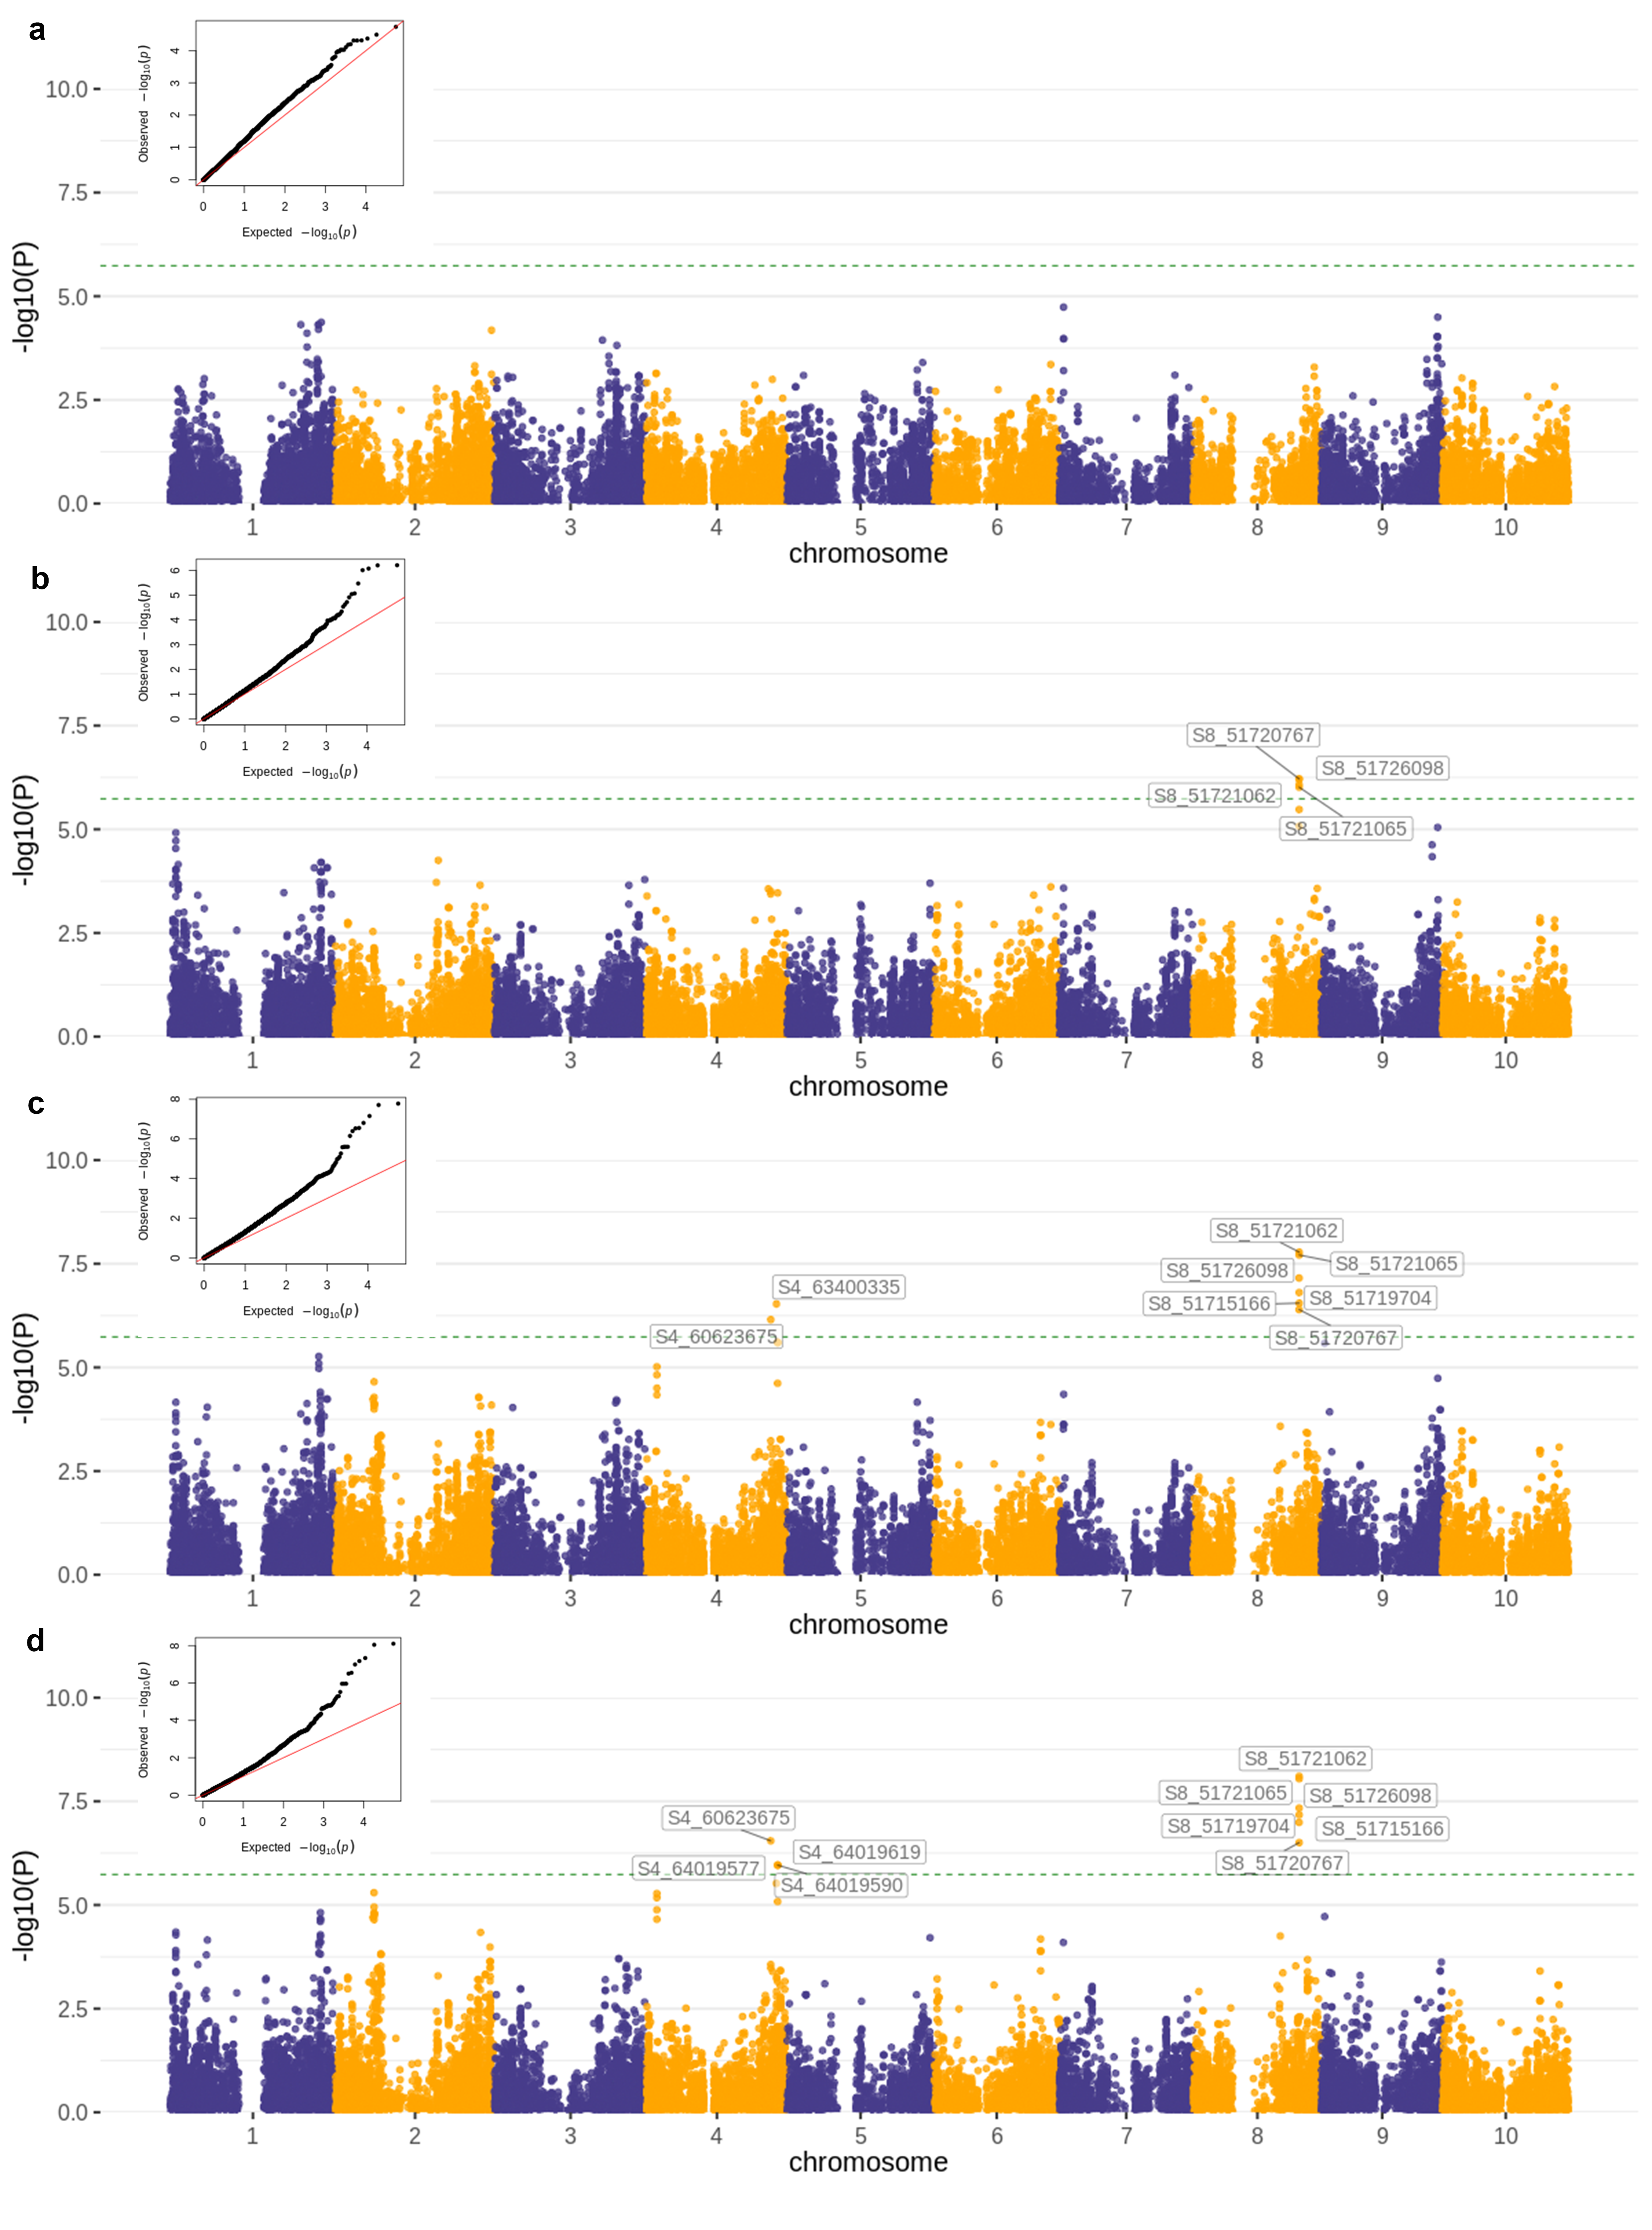
\includegraphics[width=0.95\textwidth]{Figure2}
    \caption{Manhattan plot showing genome-wide association using linear mixed model (LMM). Subfigures show univariate LMM for \textbf{a}. protein and \textbf{ b}. starch, and multivariate LMM for \textbf{c}. starch and protein. Subfigure \textbf{d}. shows univariate LMM for starch with protein as covariate. Horizontal dashed green line represents Bonferroni-corrected significance threshold for $\alpha$=0.05. Quantile-quantile plots for association analysis are presented as inset at top-left of subfigures. Significantly associated SNPs are annotated in the plots.}
    \label{fig2}
\end{figure}

\begin{figure}
    \includegraphics[width=0.7\textwidth]{Figure3}
    \caption{Linkage disequilibrium between significantly associated SNPs from chromosome 8. R-squared values to the top of the diagonal and associated p-values are at the bottom of the diagonal.}
    \label{fig3}
\end{figure}

\subsection*{Candidate genes}
We identified potential candidate genes from significantly associated SNPs based on extent of LD between SNPs in the associated regions. Since all chromosome 8 SNPs were in strong LD with each other we identified genes within the range of 51715166 bp to 51726098 bp in chromosome 8 (\textit{Supplementary Table S2}). Since chromosome 4 SNPs showed weak LD with neighboring SNPs, we identify genes within 2 Kb of the significant SNPs as potential candidate genes.
% When there were no neighboring SNPs nearby the chromosome 4 SNPs to calculate the LD statistics, we resorted to using 2 Kb average distance to avoid false positive despite the average LD decay distance for the population was approximately 20 Kb \parencite{sapkota2020}.

A total of five candidate genes had significantly associated SNPs that were within or in proximity of those genes (Table \ref{tab1}). All SNPs except one (S4\_63400335) were localized within the mRNA of the associated genes. One SNP, S8\_51715166, was located in coding sequences (CDS) of a gene encoding CASP like protein (\textit{Sobic.008G111500}), whereas, the SNPs S8\_51719704 and S8\_51726098 were situated within the CDS of a heat shock protein (HSP90-6; \textit{Sobic.008G111600}). Three signficant SNPs from $\sim$64 Mb region of chromosome 4 were located in the 3'UTR region of a Ring-H2 finger protein, \textit{Sobic.004G301300}. One SNP, S4\_60623675, was localized in the 5'UTR region of fatty acid desaturase (FAD2) gene, \textit{Sobic.004G260800}.

\begin{table}
\caption{Potential candidate genes from the significantly associated regions.}
\begin{tabular}{llllll}
\hline
Gene & Name{*} & Chr & Start & End & Associated\_SNPs \\ \hline
Sobic.004G260700 & Uncharacterized protein & 4 & 60621941 & 60622538 & S4\_60623675 \\ 
Sobic.004G260800 & FAD2 & 4 & 60623621 & 60625764 & S4\_60623675 \\ 
Sobic.004G301300 & RING-H2 finger protein & 4 & 64018712 & 64019678 & 3 SNPs\\
Sobic.008G111500 & CASP-like protein 8 & 8 & 51714673 & 51715254 & S8\_51715166 \\
Sobic.008G111600 & HSP-90-6 & 8 & 51719209 & 51726960 & 5 SNPs \\ \hline
\label{tab1}
\end{tabular}
\vspace{-0.5cm}
   \item[*]{Gene names based on annotated homologous maize genes.}.  
\end{table}

\subsection*{Gene network and expression}
We used the string-db (or whichever) to identify high confidence (0.6) first interactors of candidate genes. The two genes in chromosome 4 had a total of 10 first interactors (Fig \ref{fig4}). HSP90-6 (\textit{Sobic.008G111600}), the only chromosome 8 gene with first neighbors, had a total of 142 interactors. The gene interaction network for both sets of genes had higher number of protein-protein interaction (PPI) than expected (PPI enrichment p-value \textless 1$e^{-16}$). Gene interaction networks from chromosome 4 and chromosome 8 were sign ificantly enriched (FDR\textless 0.001) for three and six biochemical pathways, respectively (Supplementary Table S3). The chromosome 4 genes were enriched for biosynthesis of unsaturated fatty acids, fatty acid metabolism and nitrogen metabolism pathways, whereas, chromosome 8 genes were enriched for protein processing, protein export, spliceosome, endocytosis, RNA degradation, and plant-pathogen interaction. Figure \ref{fig5} shows expression atlas of chromosome 4 and chromosome 8 group of genes and interactors across various tissue types. While clear clustering of genes with differential expression across reproductive and vegetative tissues was not seen, different clusters of genes showed varying degree of transcript abundance across tissue types.

\begin{figure}
    \includegraphics[width=\textwidth]{Figure4}
    \caption{Network of candidates genes (\textit{Sobic.004G260800.1} and \textit{Sobic.004G033460.1}) and interactors from associated chromosome 4 SNPs.}
    \label{fig4}
\end{figure}

\begin{figure}
    \includegraphics[width=\textwidth]{Figure5}
    \caption{Heatmap showing gene expression analysis of interactors of candidate genes. The row colors represents chromosome 'group': purple and cyan represent chromosome 4 and 8 related genes, respectively.}
    \label{fig5}
\end{figure}

The FAD2 gene (\textit{Sobic.004G260800}) in chromosome 4 interacted with another fatty acid desaturase gene (DES2, \textit{Sobic.004G260600}) which is located $\sim$570 Kb upstream from the FAD2 gene. Both FAD2 and DES2 strongly interact with three nitrate reductase (NADH) genes, two of which located in chromosome 4 at $\sim$55 Mb (\textit{Sobic.004G196101}) and $\sim$65 Mb (\textit{Sobic.004G312500}) while the other is located around 58-59 Mb in chromosome 7 (\textit{Sobic.007G153900}) (Figure \ref{fig4}). The FAD2 gene was highly expressed in flower, embryo and shoot, whereas, its interactor DES2 had higher expression in root tissues (Fig \ref{fig6}). The heat shock proteins are known to be molecular chaperones primarily involved in drought and stress response but can also be involved in other molecular processes during plant development \parencite{yu1998polypeptides,khan2019heat}. The gene expression results showed HSP-90 (\textit{Sobic.008G111600}) to be highly expressed in floral meristem, plant embryo and vegetative meristem compared to root, shoot, and flower tissues (Fig \ref{fig6}). The interactors of HSP90-6 included several HSP70 genes which were also highly expressed in reproductive tissues compared to root and shoot tissues (Fig \ref{fig6}).

\begin{figure}
    \includegraphics[width=\textwidth]{Figure6}
    \caption{Gene expression of candidate genes and some of their interactors. X-axis represents various tissue types, and y-axis shows relative expression (TPM: transcript per million). HSP: heat shock protein, FAD/DES: fatty acid desaturase, NADH: nitrate reductase.}
    \label{fig6}
\end{figure}
% The string results for \href{https://string-db.org/cgi/network.pl?taskId=4w6ogQsNLgPQ}{chromosome 8} and \href{https://string-db.org/cgi/network.pl?taskId=sGUWcEEzwMCO}{chromosome 4} gene interaction network. 

% 1. How starch and protein differ between different subpopulations?
% 8. Haplogroup analysis: 
%  a. Phenotypic variation based on haplotypes/LD for genes (start with the ones in CDS).
%  b. Functions and putative protein conformation changes for those genes.
%  c. Gene expression profile for those genes.
% ** VIT genes and the significant hits near it. Look at haplotypes between sweet and unsweet. Also between other lines with different phenotypic variability.
% Chr4 - 1Kb: Sobic.004G247200 is the one that has interaction (>700)
% Chr8 - range: Sobic.008G111600 is the interactor (>700) > 79 interactors
% Some interactors couldn't be used in gene expression analysis because they didn't convert to the new version.

\section*{Discussion}
Despite being two of the most studied grain quality phenotypes, large proportion of genetic variance in starch and protein remains unexplained. In this study, we aimed to identify genetic loci associated with starch and protein content in sorghum grain. We observed strong genotypic effect and some genotype $\times$ environment effect for starch and protein in our population (Supplementary Table S1). Previous studies have also reported high heritability for starch and protein in different populations \parencite{rami1998quantitative,murray2008genetic,rhodes2017genetic}.

In our genome-wide association study, we used only the random genetic effects (BLUPs) to identify marker trait association for strictly genetic effects. The lack of genetic association for protein content could be due to smaller genetic effects and larger environmental effects on this trait. Starch, with no environmental effect and larger genotypic effects, had genetic variants significantly associated with the phenotype. Five SNPs (in strong LD with each other) from a single locus that encodes for a heat shock protein (HSP) 90 (\textit{Sobic.008G111600}), with two SNPs located on the coding sequence, showed significant association. This loci was not identified during association mapping of starch in previous studies using this population \parencite{rhodes2017genetic,boyles2017genetic}. HSPs are common group of protein found in eukaryotes and function as molecular chaperones that help in refolding proteins denatured by heat and keep them from aggregating \parencite{vierling1991roles,boston1996molecular}. Two distinct members of the Hsp70 family of stress-related protein were localized in the maize amyloplast and form transient complexes with starch synthase 1 (SSI) and other stromal enzymes \parencite{yu1998polypeptides}. In Japanese sake-brewing rice rich in starch content, the HSP70 protein was highly abundant in amyloplast compared to cytosol and its concentration was elevated during the later stages of grain development \parencite{kamara2009japanese}. The HSP90 gene in this study was seen to be strongly interacting with numerous molecular chaperones including HSP70. Since the HSP90 and interacting HSP70 proteins showed higher expression in the embryo and floral meristem compared to root and shoot tissues, they are likely important candidates responsible for protein processing and export during grain filling in sorghum.

For complex traits, understanding if a genetic variant affects multiple phenotypes simultaneously (pleiotropy) or affects one phenotype through affecting another phenotype is one of the major challenge \parencite{yang2012methods}. Starch and protein constitute most of the grain composition and display a strong negative correlation. We identified additional marker trait associations when: 1) starch and protein were fit as dependent variables in a multivariate mixed model, or 2) when protein was fit as independent variable for a model with starch as dependent variable. This approach helped us identify an important variant, S4\_60623675, which showed significant association in both of the above mentioned models and was located in the 5' UTR of a fatty acid desaturase gene (\textit{Sobic.004G260800}). The fatty acid desaturase gene interacted with two more desaturase genes and three nitrate reductase genes, forming a network that is highly enriched for biochemical pathways for fatty acid and nitrogen. One of the interacting desaturase gene (DES2, \textit{Sobic.004G260600}) is involved in the biosynthesis of aliphatic side chain of sorgoleone by converting palmitoleic acid to hexadecadienoic acid \parencite{pan2007functional}. Sorgoleone is a phytotoxic secondary metabolite that plays a direct role in allelopathic interactions. Sorgoleone is known to inhibit photosynthesis, but the relationship between Sorgoleone biosynthesis pathway and seed development is unclear  \parencite{einhellig1993effects}. \citet{rhodes2017genetic} has previously reported significantly associated variants for protein and fat around 57-58 Mb of chromosome 4 which is $\sim$2-3 Mb from our associated SNPs. The high expression of HSP90 gene in plant embryo combined with a candidate SNPs in the fatty acid desaturase gene identified using MV-LMM hints at possible connection between the biochemical pathways for starch, protein and fat content during grain development. The enrichment of biochemical pathways involving these genes and their high expression in reproductive tissues warrants further characterization and functional analysis of these candidates.

In conclusion, we were able to identify a previously uncharacterized genomic region associated with starch content using univariate LMM. The genomic region harbored a heat shock protein which shows strong protein-protein interaction and its network is enriched for several biochemical pathways. Additionally, we also showed that use of MV-LMM for correlated traits can help identify additional genomic regions that go undetected with the univariate GWAS of single traits. The candidates of this study might be involved in intricate metabolic pathway and represent possible pleiotropic targets for source-sink activities during grain filling.


\section*{Supporting Information}
Supplementary information is included in Appendix C.

\section*{Data availability}
The codes and data used in the study are available at \href{https://github.com/sirjansapkota/StarchProtein}{github.com/sirjansapkota/StarchProtein}.
% If you intend to keep supporting files separately you can do so and just provide figure captions here. Optionally make clicky links to the online file using \verb!\href{url}{description}!.

%These commands reset the figure counter and add "S" to the figure caption (e.g. "Figure S1"). This is in case you want to add actual figures and not just captions.
\setcounter{figure}{0}
\renewcommand{\thefigure}{\arabic{figure}}

% % You can use the \nameref{label} command to cite supporting items in the text.
% \subsection*{S1 Figure}
% \label{example_label}
% {\bf Caption of Figure S1.} \textbf{A}, If you want to reference supporting figures in the text, use the \verb!\nameref{}!. command. This will reference the section's heading: \nameref{example_label}.

% \subsection*{S2 Video}
% \label{example_video}
% {\bf Example Video.} Use \href{www.youtube.com}{clicky links} to the online sources of the files.

% %\clearpage

% \nolinenumbers

%This is where your bibliography is generated. Make sure that your .bib file is actually called library.bib
\printbibliography

% \begin{thebibliography}{10}

% %This defines the bibliographies style. Search online for a list of available styles.

\end{document}

